%%==========================
%% chapter01.tex for SJTU Master Thesis
%% based on CASthesis
%% modified by wei.jianwen@gmail.com
%% version: 0.3a
%% Encoding: UTF-8
%% last update: Dec 5th, 2010
%%==================================================

%\bibliographystyle{sjtu2} %[此处用于每章都生产参考文献]
\chapter{绪论}
\label{chap:Intorduction}

程序分析是近年来的热门话题,而其中利用工具搜集和分析程序动态运行时的信息的技术也被广泛采用。另一方面,随着计算机硬件的发展,多核、分布式技术的适用范围和效率也越来越高,并行程序的重要性也逐渐凸显。本文结合了动态程序分析的特点,将动态程序分析与并行化结合起来,提出并开发了一个适用于编写并行的动态分析程序的框架,并通过实验证明了该框架的实用性和效率。

\section{研究背景}

近年来,随着编程技术和研究的深入,越来越多的语言特性被编程者们所开发和采用,多态、反射、动态加载等技术的使用也越来越广泛。而这些技术对采用对传统的静态编译和分析提出了挑战。污点分析\cite{taint01,taint02}和符号执行\cite{symbExec}等静态分析的方法由于分析效率较低,加之难以收集程序动态运行时的一些信息,其局限性逐渐凸显。为了解决这些问题,动态分析的技术被引入。顾名思义,动态分析即是在运行被分析程序的状态下运行分析程序,从而能够有效地减少分析规模,提高分析精度,并能收集动态信息。一些静态分析技术如程序切片\cite{dynSlc}和符号执行\cite{dynSym}也相应地加入了动态分析的内容。

动态程序的分析有效地减少了相对分析时间,但实际在面对重量级分析的时候,整个分析过程所消耗的时间依然很多,尤其是面对一些本身比较庞大、复杂的程序,在算法已经经过优化的情况下仍旧不能有效地提高运行效率的时候,每个测试用例或者被分析程序动辄需要运行几个小时乃至几天,给程序的分析、查错和优化带了了很大的不便。基于该问题,研究者们采取了不同的解决方案。除了在分析方法本身进行改进分析和在算法的效率以及复杂度上作提高之外,也有另一些方案针对分析程序的执行作加速,其中就包括了并行化的方法。

\section{并行程序分析}

并行化是基于多核、分布式技术等多种硬件技术的发明及成熟而发展起来的技术。在传统的串行计算中,指令是顺序串行执行的,即便后续指令没有用到之前的指令的结果,也只能进行等待,造成了时间上的浪费。并行的理念就是将这些并行度大的指令或者任务派发给空闲的计算资源如cpu核心、物理机等进行分开处理,从而提高计算效率。

在动态程序分析方面,有一些程序所采用的的分析内容也具有这种并行性。这些分析程序只是从所运行的被分析程序处取得相关的运行信息,然后进行处理。这些分析程序一般没有返回值,或者不需要写回被分析的程序。换言之,这些分析程序对被分析程序基本没有影响。一个简单的例子就是函数计数。函数计数旨在计算程序动态运行时一共执行了多少函数,进一步拓展还可以分析每个函数各执行了多少次,每次花费了多少时间,从而给使用者优化和调试提供有效信息。如\ref{fig:dig1}所示,我们可以看到,每次执行一个函数之后,被分析程序调用Count()函数,事实上就是把计数器作加一的处理。Count()函数只是被动接受调用,然后对一个与被分析程序无关的计数器写入值,并没有影响到被分析程序本身,故而该方法可以进行并行化。

\begin{figure}[!htp]
  \centering
  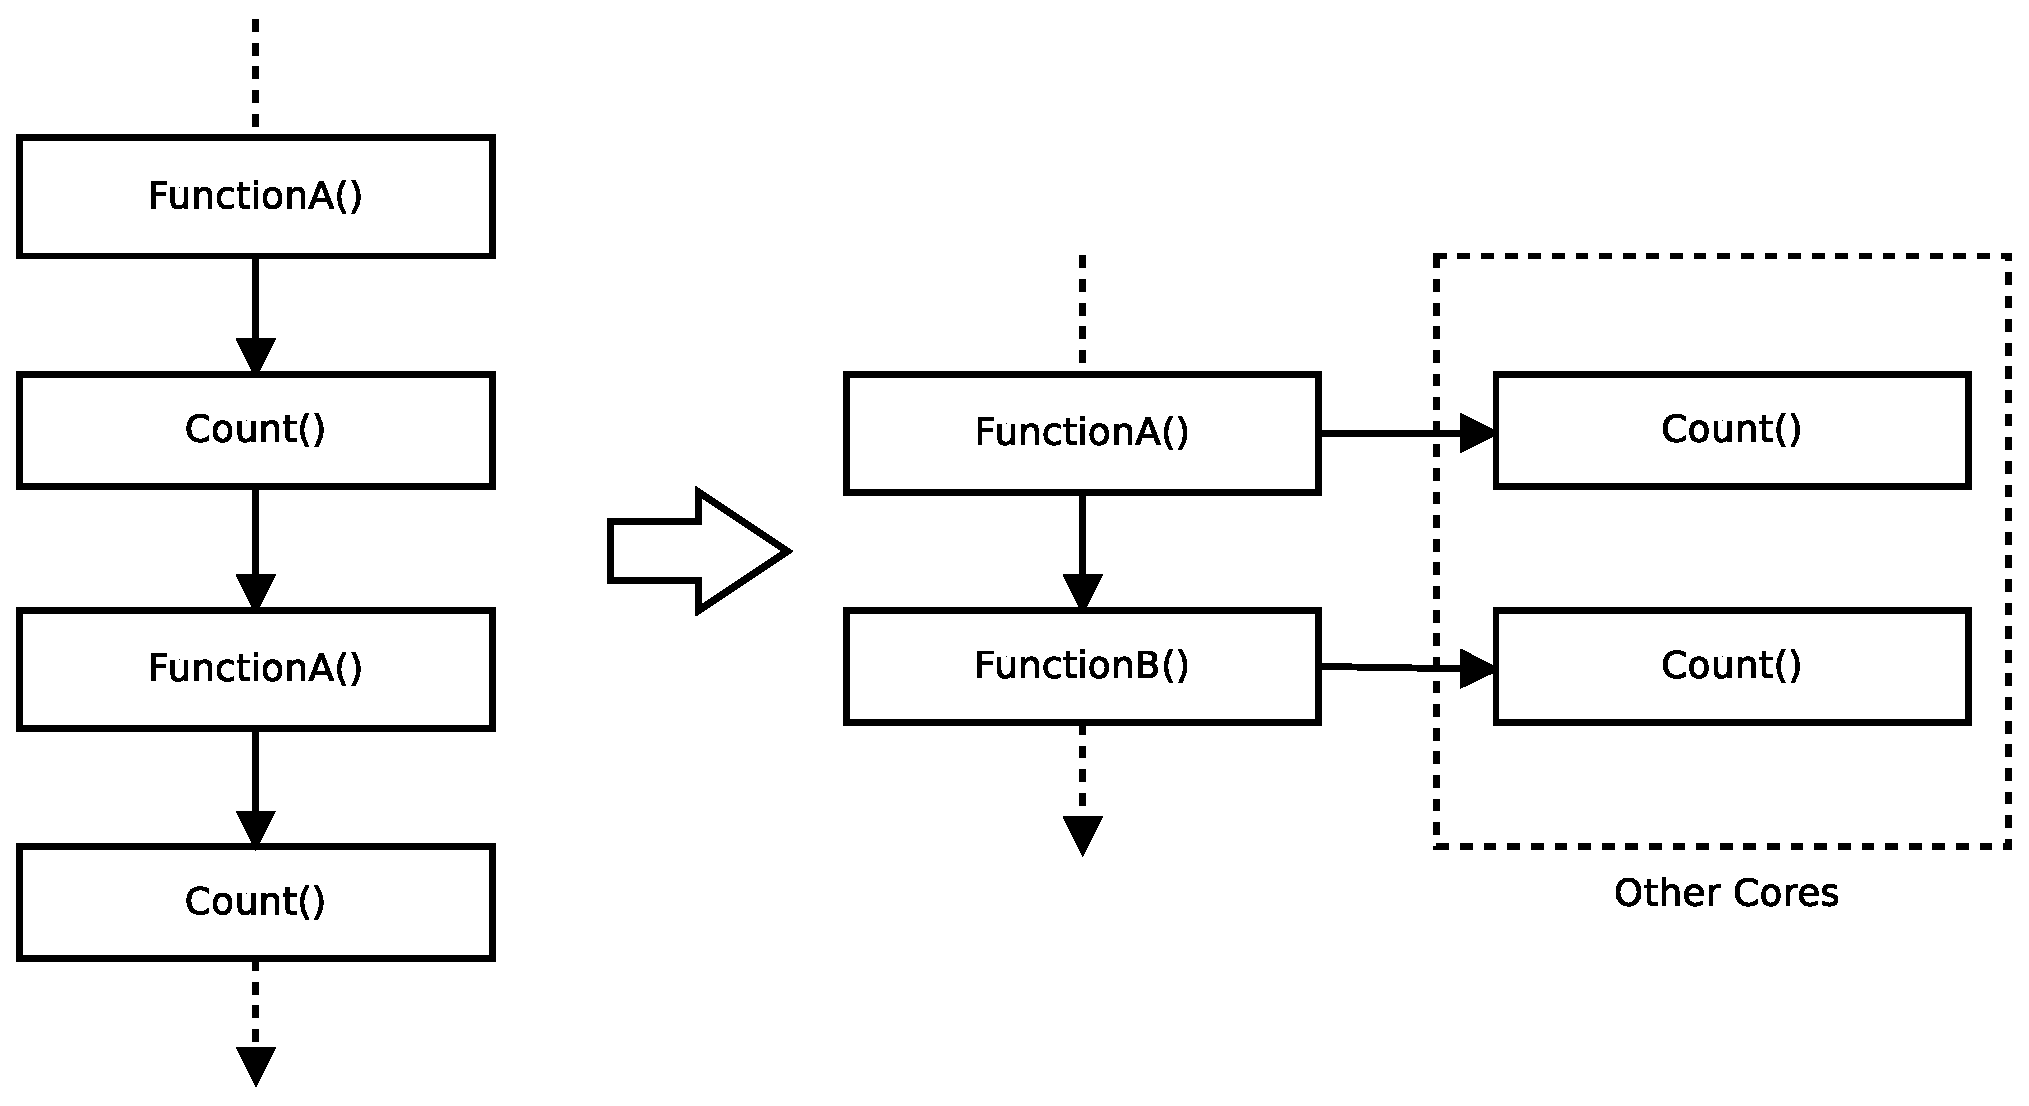
\includegraphics[width=0.8\textwidth]{chap1/Dig1}
  \bicaption[fig:dig1]{函数计数的简单例子}{函数计数的简单例子}{Table}{A simple example of method count}
\end{figure}

与此类似,很多其他的分析程序也可以进行并行化的处理。文献\cite{paSpeed}中指出,在串行执行的情况下,二进制动态程序分析可能会导致高达1000倍缓慢的速度。这是会很大程度上影响到被分析程序本身的。因此,将分析程序与被分析程序分离开来执行,理论上能提升动态分析的效率。

\section{已有解决方案}

Shadow profiling\cite{shaPro}是采用并行化进行程序分析的一个方案。不同于以往串行执行中直接一起执行分析程序与被分析程序,它创建了一个处理的线程,称为影子线程,专门用于处理和执行分析程序。由于利用了现代操作系统里基于拷贝的创建子进程操作,Shadow profiling中的处理线程可以认为是父线程(即被分析程序)的一个拷贝。但由于采用这种方式,各个线程之间是共享地址空间的,故而在程序安全方面不能得到保证。

Superpin\cite{superPin}则是另一个比较有名的动态并行程序分析框架,它采用了Pin作为动态注入的工具,在此基础上进行并行化的处理。与Shadow profiling不同的是,Superpin是将被分析程序以时间片为单位进行切分,通过对这些时间片以拷贝进程的方式进行并行,从而达到提高效率的效果。由于父线程即被分析程序没有引入很多的负载,所以可以全速运行,而子进程则相应地执行相关的并行任务。每个时间片都有相应的开始信号和停止信号,用以完成CPU之间的同步和任务的交付。这个框架主要有几个方面的问题需要考虑:

\begin{itemize}
	\item 任务之间的时序和同步。各个任务在原程序中是以一定的时序执行的,如何保证在并行执行的过程中这些任务仍以一定的顺序执行而不产生同步问题或者结果出错是一个问题。
	\item 系统调用的问题。父线程和子线程中对系统调用的处理必须保持一致性。
	\item 超时问题。由于采用了多线程和时间切片的方式,所以时序同步十分重要,应该正确处理好超时等情况。
	\item 侦测签名/时间戳的问题。该系统采用了一个唯一的签名作为一个时间切片开始的标志,从而使得系统状态得以被描述,从而使得时间切片间不会出现不合理的重叠,从而打乱执行顺序。
	\item 结果合并。并行的结果分别由不同的线程得出,此时各个线程的结果需要进行合并。
\end{itemize}

Trident\cite{eventDri}与前两者相比,采用了硬件支持的解决方案。通过采用事件驱动,它能有效地发现程序运行时所存在的优化的可能性,然后使用空闲线程对原程序进行动态优化,从而有效地提高整个程序的效率。硬件辅助的引入,使得这个发现的过程更加高效,减少了对主线程的开销。但相比于前两者,该工具只是进行了并行的动态优化,实质上整个原程序仍然是没有并行执行的。

\section{本文的解决方案}

在以往的解决方案中,并行进行程序分析的主要思想在于将对被分析程序没有影响的一些分析任务与被分析程序分离开来,使用空闲的线程和计算资源进行并行处理。但是该分离过程需要参数传递,线程创建,函数调用等过程。如果是细颗粒的一些任务,在并行处理的过程中,调用的次数会相对频繁很多,造成的结果就是多次调用造成的开销变多。

例如在Java中,如果我们以方法为单位进行并行分析,意即一个方法是一个分析任务,每次遇到分析点的时候即调用相关的方法进行处理,此时主线程即被分析程序就可以继续执行下去,分析程序被交付给其他的处理线程进行处理,从而能提高程序分析的效率。理论上这个方法是可行而且高效的,但在实际应用中,线程间的通信,沟通和同步所花费的开销就要大很多了。

还是以之前的函数计数为例。例如我们需要计算整个Java程序执行的过程中一共执行了多少个方法,其中方法Count()被插桩在被分析程序的每个方法入口,一旦被调用,则往计数器执行加一的操作,直至程序运行结束,返回计数器值,就是执行的函数总数了。在这个例子中,未插桩之前的程序就是被分析程序,而Count()方法就是分析程序。如果被分析程序是个比较庞大的程序,那么Count()方法就会被调用很多次,可能是几千甚至上万次。在这个情况下如果我们采用简单的并行的方法,那么整个完成并行的过程就需要相应次数的参数传递、进程间通信等过程;另一方面,由于Count()本身是完成对计数器加一的操作,因而是一个比较轻量级的操作,每次执行的开销并不算大。这两个因素造成的一个结果就是并行处理之后的程序在效率上有的时候并没有比原程序高,相反反而降低了。

为了解决这种情况,本文的解决方案基于另一种新的解决方案,即基于缓存机制的程序并行化框架。需要被并行的方法并不会在执行的时候立即交付给并行线程进行处理,而是先缓存起来,等到累计到了一定的数量的时候,才一起交付。在这种情况下,本来需要进行多次的进程间通信被缩减为一次,从而降低了在构建并行线程的时候的开销。在该方案的基础上,本文对其进行了一些相关的优化。

\section{本章小结}

本章阐述了程序分析技术的进步,并指出了一些程序分析技术在效率上的不足,并提出了通过并行化来解决这一问题的一个方案。接下来介绍了几个比较有名的工具和框架,并比较了他们在并行化处理程序分析上的一些异同。最后本文阐述了以往并行框架存在的一些确定,并提出了相应的解决方案。

% PiPA\cite{pipa}是一种现有的并行化程序分析的方案,它采用了DynamoRIO作为二进制动态代码插桩工具来生成并行代码
